\section{Heat Removal from Reactor}

\subsection{General Thermodynamics Considerations}

\subsubsection*{Design Principles}

\begin{enumerate}
    \item Fuel maximum temperature < its melting temperature at corresponding burn-up ($2200 - 2450 {}^{\circ}{\rm C}$)
    \item No boiling crisis (MDNBR > 1.3)
    \item Sufficient cooling
    \item No flow instability
\end{enumerate}

\subsubsection*{Nuclear Limits}

\begin{enumerate}
    \item Hot spot factor
    \begin{itemize}
        \item Peak power in pin
        \item Prevent fuel melting
    \end{itemize}
    \item Hot channel factor
    \begin{itemize}
        \item Assure heat removal from pin
        \item MDNBR: Minimum Departure from Nucleate Boiling Ratio
    \end{itemize}
    \item Design considerations
    \begin{itemize}
        \item Limits on power
        \item Materials
    \end{itemize}
\end{enumerate}

\subsubsection*{Heat Removing}

\begin{itemize}
    \item Fuel pin power production
    \begin{itemize}
        \item Heat conduction
        \item Fourier law
        \item Poisson's equation
    \end{itemize}
    \item Gap to clad: Heat conduction
    \item Clad heat transfer: Poisson's equation (no heat source)
    \item Clad to coolant: Newton's law of cooling
\end{itemize}

When heat is added to a substance at constant pressure, essentially all of the heat is used to increase its enthalpy.

\subsection{Heat Generation in Reactors}

\subsubsection*{Energy Released in Fission}

For the fission of ${}^{235}{\rm U}$, 

\begin{itemize}
    \item More than 90\% of the recoverable fission energy deposited in the fuel rods
    \item About 5\% deposited in the moderator
    \item Less than 5\% deposited in the blanket, reflector, and shield
\end{itemize}

\subsubsection*{Power Distribution}

According to the {\itshape Uniform Bare Pile} hypothesis, the heat release rate per unit volume is a cosine function distribution in axial direction and a zero-order Bessel function distribution in radial direction.

\subsubsection*{Fission Products Decay Heating}

\begin{itemize}
    \item About 7\% of the total thermal power output of the reactor
    \item Due to the Fission Products decaying heat, a means for cooling the reactor core after shutdown must be provided in all reactors
\end{itemize}

\subsection{Heat Conduction}

\begin{definition}
    Heat is transmitted from one location in a body to another as a result of a temperature difference existing in body (there is no macroscopic movement of any portion of body).
\end{definition}

Differential equation of heat conduction: 
\begin{equation}
    \rho c_p \pdv{t}{\tau} = \nabla \cdot \kappa \nabla t + q_v
\end{equation}

\subsection{Heat Transfer to Coolant}

\begin{definition}
    Heat is transferred to a moving liquid or gas, as the result of a temperature difference as well.
\end{definition}

Newton's law of cooling: 
\begin{equation}
    q = h \Delta t
\end{equation}

Influent factors of $h$: 
\begin{itemize}
    \item Cause of flow
    \item Phase transition of fluid
    \item The flow state of a fluid (Laminar or Turbulent Flow )
    \item Geometric factor
    \item Nature of the coolant fluid
\end{itemize}

Most of the heat produced in the fuel flows directly to the coolant in a direction normal to the axis of the fuel rod.

Equivalent Diameter
\begin{equation}
    D_{\rm e} = \frac{4A}{P_w} = \frac{4\times \text{cross-sectional area of coolant channel}}{\text{wetted perimeter of coolant channel}}
\end{equation}

For liquid metals, it is strikingly different from ordinary coolants, 
\begin{enumerate}
    \item High thermal conductivity
    \begin{equation}
        \kappa_{\rm Na} = 122 \kappa_{\rm H_2 O}
    \end{equation}
    \item Heat conduction dominates heat transfer even in turbulent flow
\end{enumerate}

\subsection{Boiling Heat Transfer}

Distinct advantages
\begin{enumerate}
    \item The coolant pressure is much lower
    \item Require lower cladding and fuel temperature for a given flow rate and heat flux
\end{enumerate}

\begin{tip}
    PWR permits boiling of restricted nature.
\end{tip}

\subsubsection*{Boiling Heat Transfer Curve of Large Volume}

\begin{figure}[H]
    \centering
    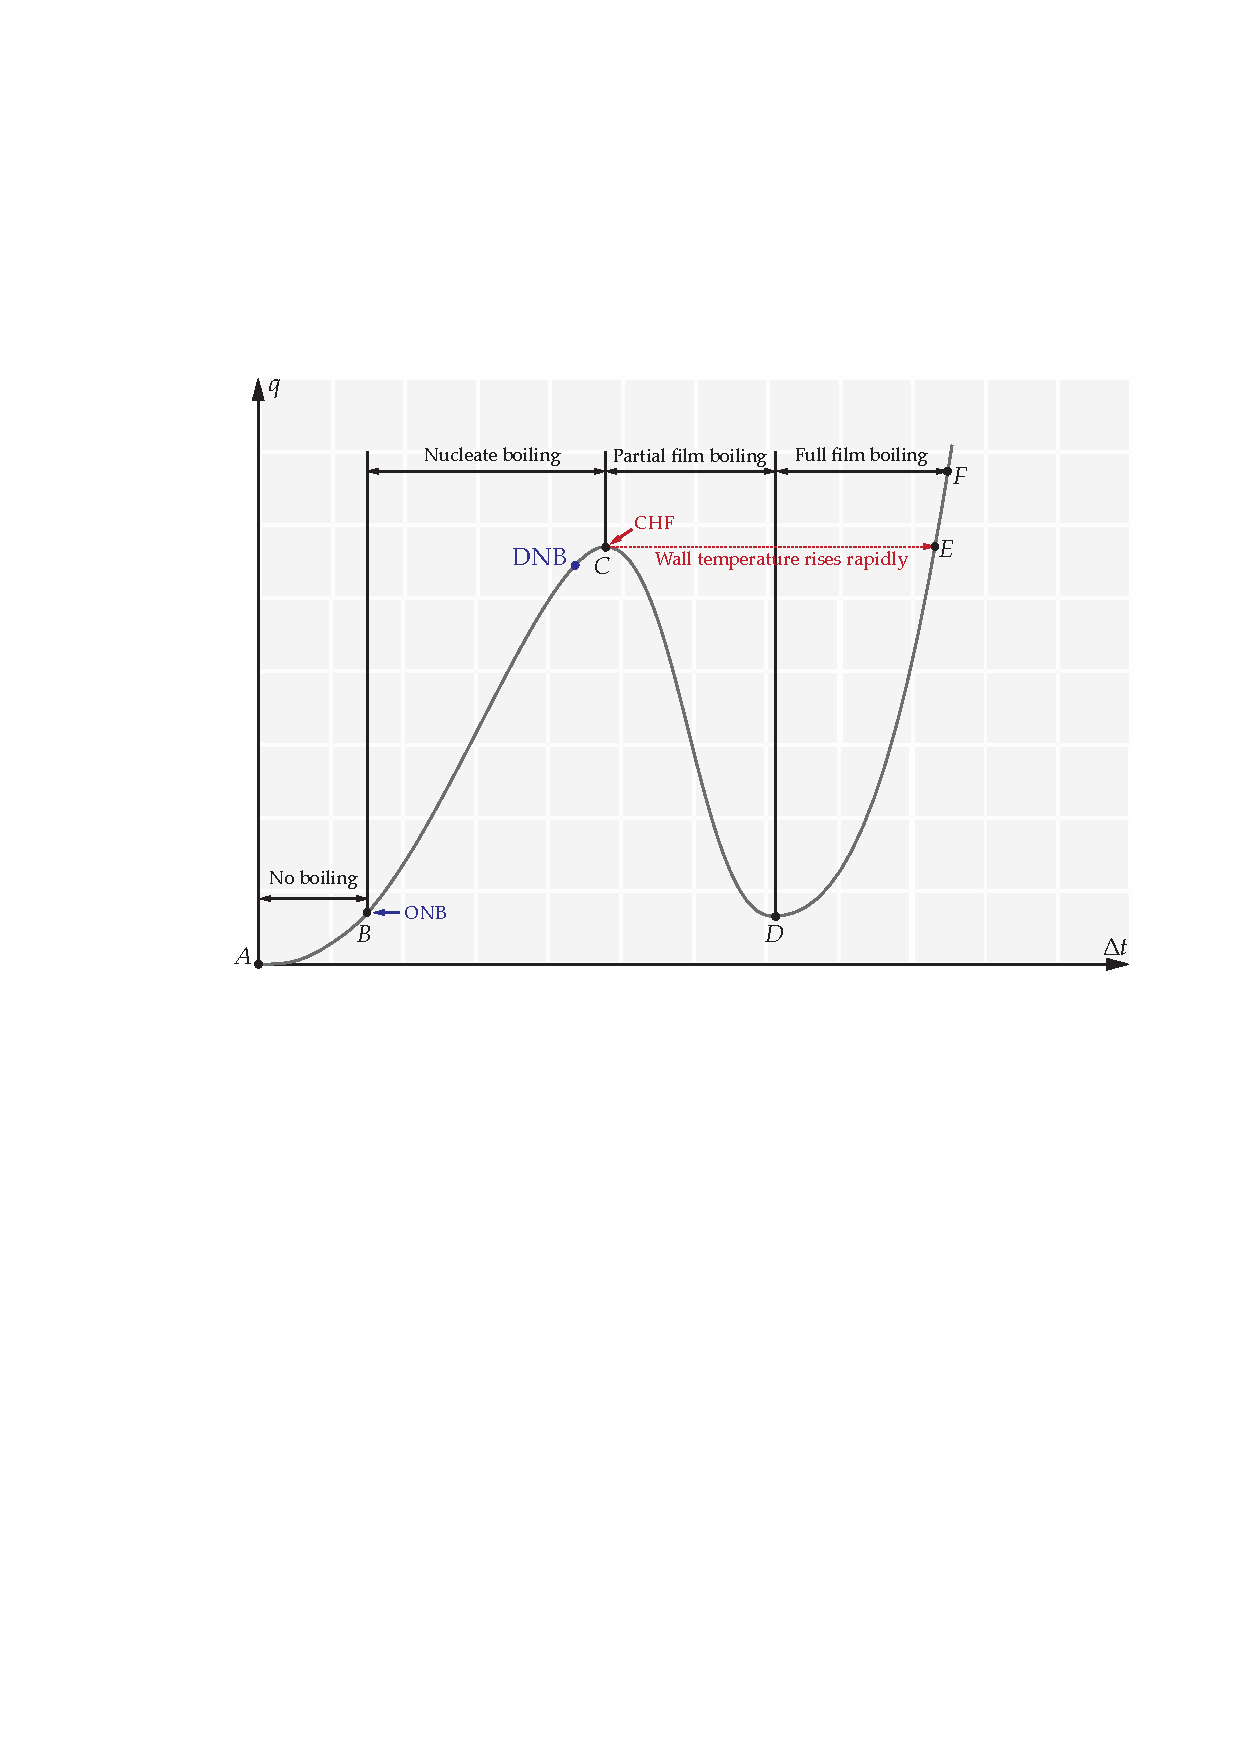
\includegraphics[scale=0.6]{figures/boiling_curve.pdf}
    \caption{Boiling Heat Transfer Curve of Large Volume78694532 }
\end{figure}

\subsection{Thermal Design of a Reactor}

\begin{enumerate}
    \item Determine the thermal parameters
    \item Fuel rod parameters
    \item compute $\Delta p$, MDNBR, $t$ and so on
    \item Technical and economic evaluation
    \item Thermal and hydraulic experiment
\end{enumerate}